Примеры построения графиков равномерного и нормального распределения приведены на рисунках \ref{pic:eval} и \ref{pic:norm}.

\begin{figure}[h]
	\begin{center}
		{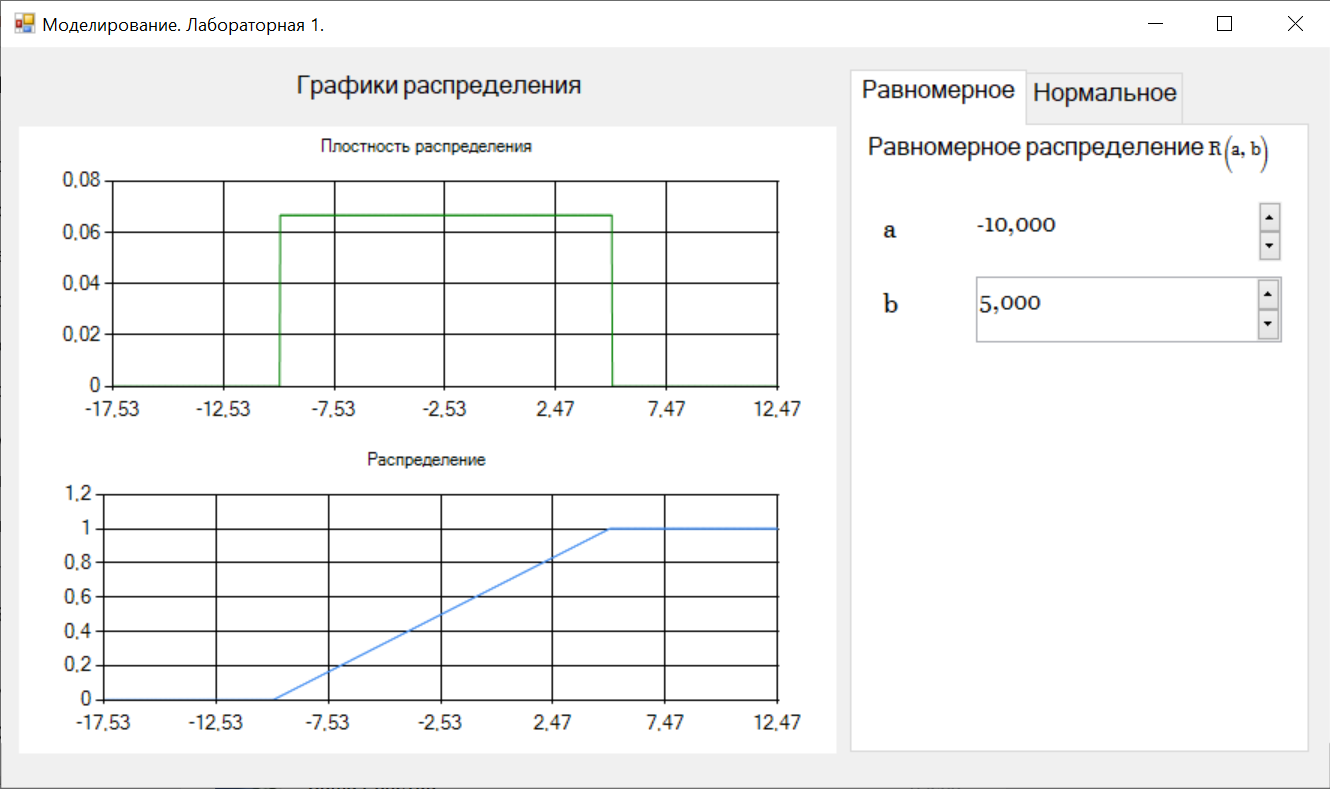
\includegraphics[scale=0.7]{EvalDist}}
		\caption{Графики распределения и плотности распределения для равномерного распределения}
		\label{pic:eval}
	\end{center}
\end{figure}

\begin{figure}[h]
	\begin{center}
		{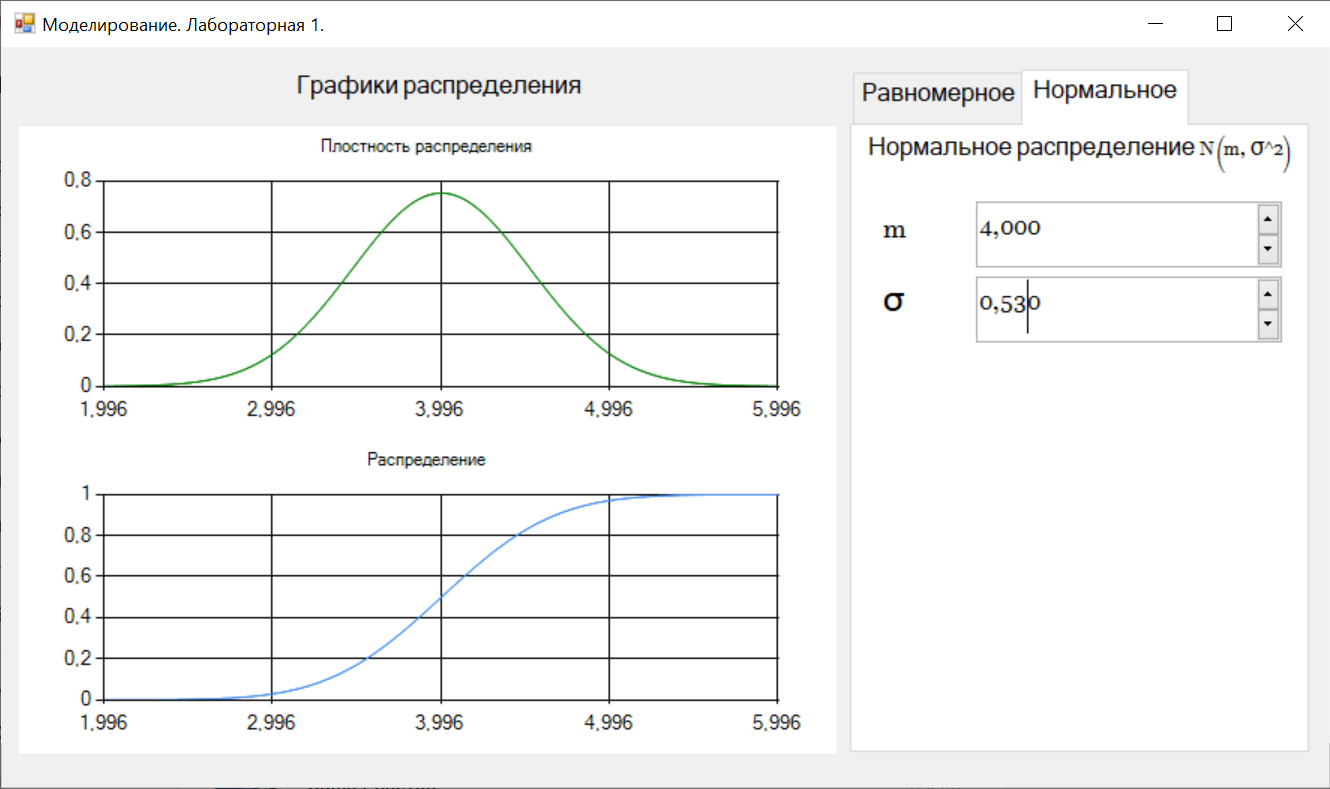
\includegraphics[scale=0.7]{NormDist}}
		\caption{Графики распределения и плотности распределения для нормального распределения}
		\label{pic:norm}
	\end{center}
\end{figure}